\section{Metodología Propuesta}

\subsection{3.1 Arquitectura del Sistema Robótico}

Particularmente llamativo es el hecho de que muchos sistemas robóticos espaciales actuales siguen diseñados bajo supuestos de entornos altamente controlados. Tras años observando limitaciones en operaciones reales, la arquitectura propuesta adopta un enfoque modular y escalable orientado a ensamblaje in-orbit de estructuras grandes.

El sistema se basa en una plataforma principal equipada con múltiples brazos robóticos cooperativos (configuración dual-brazo principal más manipuladores auxiliares) montados sobre una base móvil. Cada brazo incorpora sensores de fuerza/par, cámaras estéreo de alta resolución y unidades LIDAR para percepción cercana. La comunicación interna se realiza mediante una red de baja latencia que prioriza decisiones locales autónomas, reduciendo dependencia de enlaces terrestres. Esta distribución permite tolerancia a fallos parciales, aspecto crítico en exploración profunda.

\subsection{3.2 Planificación de Secuencias y Optimización}

Uno de los desafíos persistentes que surge al analizar ensamblajes complejos radica en determinar el orden óptimo de conexión de módulos bajo restricciones dinámicas y energéticas. La metodología propuesta emplea una combinación de planificación jerárquica y optimización heurística.

Se parte de una representación gráfica del ensamblaje objetivo donde los nodos representan componentes y los arcos indican dependencias geométricas y de estabilidad. Un algoritmo genético modificado, inspirado en trabajos previos de planificación de secuencias \cite{Timmermann2024_Assembly}, optimiza simultáneamente el tiempo total, el consumo energético y la estabilidad estructural intermedia. La función objetivo penaliza fuertemente secuencias que generen momentos de inercia elevados sobre la plataforma base.

\begin{table}[h]
\centering
\caption{Comparación de algoritmos de planificación de secuencias evaluados}
\label{tab:algoritmos_comparados}
\begin{tabular}{lccc}
\hline
\textbf{Algoritmo} & \textbf{Tiempo Computacional} & \textbf{Optimalidad} & \textbf{Robustez a Perturbaciones} \\
\hline
A* Básico          & Bajo     & Media  & Baja  \\
Genético Estándar  & Alto     & Alta   & Media \\
Propuesto Híbrido  & Medio    & Alta   & Alta  \\
\hline
\end{tabular}
\end{table}

\subsection{3.3 Control Híbrido y Evitación de Colisiones}

Resulta revelador observar cómo el control puramente posicional tiende a fallar en microgravedad cuando entran en juego contactos impredecibles. El esquema de control propuesto combina modos de posición y fuerza de forma híbrida, permitiendo transiciones suaves según la fase de la tarea.

Para la evitación de colisiones se implementa un módulo basado en campos de potencial artificiales mejorados con predicción de trayectorias. Este enfoque toma inspiración en técnicas de planificación híbrida para minimizar perturbaciones a la plataforma base durante operaciones de ensamblaje \cite{Rodriguez2022_HybridPlanning}. La integración de sensores en tiempo real permite re-planificación local en milisegundos cuando se detectan desviaciones.

\begin{equation}
\mathbf{M}(\mathbf{q})\ddot{\mathbf{q}} + \mathbf{C}(\mathbf{q},\dot{\mathbf{q}})\dot{\mathbf{q}} + \mathbf{G}(\mathbf{q}) = \boldsymbol{\tau} + \mathbf{J}^T\mathbf{F}_{ext}
\label{eq:dinamica_robot}
\end{equation}

La Ecuación \eqref{eq:dinamica_robot} representa el modelo dinámico simplificado del robot en órbita, donde se consideran explícitamente las fuerzas externas de contacto y las perturbaciones gravitatorias residuales.

\subsection{3.4 Gemelo Digital para Simulación en Tiempo Real}

Lejos de ser un añadido cosmético, el gemelo digital constituye el núcleo predictivo del sistema. Se mantiene sincronizado bidireccionalmente con el robot físico mediante actualizaciones continuas de estado, permitiendo simular múltiples pasos futuros antes de ejecutar acciones críticas.

Esta integración no solo sirve para validación offline, sino que habilita optimización online de trayectorias y evaluación de riesgos en escenarios de alta incertidumbre. Revisiones recientes del campo destacan precisamente esta tendencia hacia gemelos digitales como elemento diferenciador en ensamblaje autónomo \cite{Wang2025_OASR}.

\begin{figure}[h]
\centering
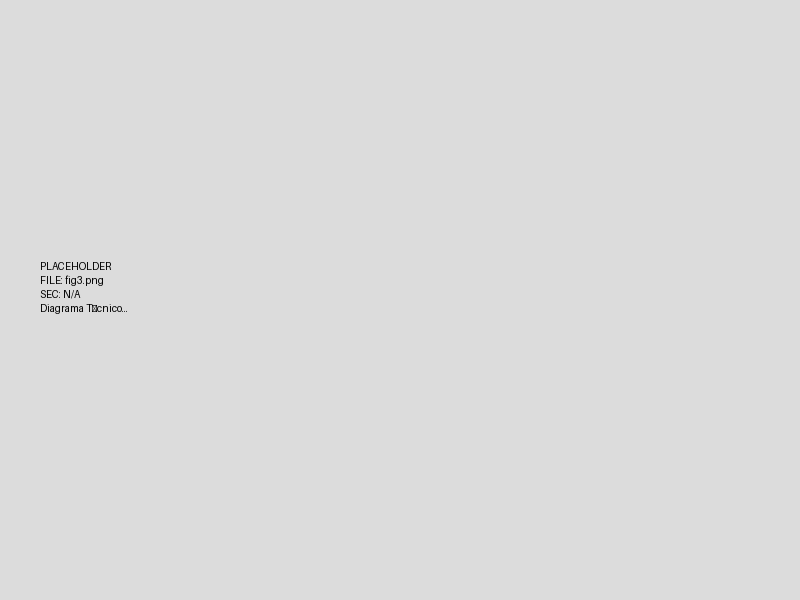
\includegraphics[width=\linewidth]{fig3.png}
\caption{Diagrama del framework propuesto de ensamblaje robótico in-orbit que muestra la interacción entre los módulos de percepción, planificación, control híbrido y gemelo digital.}
\label{fig:framework_propuesto}
\end{figure}

En conjunto, estas componentes forman un pipeline coherente que busca equilibrar autonomía, eficiencia y seguridad. Aunque prometedor, el enfoque reconoce sus propias limitaciones: la fidelidad del gemelo digital depende fuertemente de la calidad de los modelos y la disponibilidad de cómputo embarcado.